\documentclass{article}
\usepackage{enumitem,amssymb}
\newlist{todolist}{itemize}{2}
\setlist[todolist]{label=$\square$}
\usepackage{hyperref}
\hypersetup{
	colorlinks=true,
	linkcolor=blue,
	filecolor=magenta,      
	urlcolor=cyan,
	pdftitle={Overleaf Example},
	pdfpagemode=FullScreen,
}
\usepackage{graphicx}
\usepackage[margin=0.75in,headsep=.2in]{geometry}


\usepackage[svgnames,table]{xcolor}
\usepackage[tableposition=above]{caption}
\usepackage{pifont}

\newcommand*\CHECK{\ding{51}}

\begin{document}
	
{\huge \textbf{Kinetic Systems Class VERSIONNUMBER}}

\vspace{1cm}

{\huge \textbf{Vocabulary Sheet}}

\begin{itemize}
  \item \textbf{Git} - A Version Control System for managing text files
  \item \textbf{GitHub} - A website where git repositories are shared
  \item \textbf{Repository} - A collection of files and their save-points
  \item \textbf{Github Project} - A collection of repositories 
  \item \textbf{Repository Fork} - A copy of a repository that you can edit
  \item \textbf{Pull Request} - A request to bring changes from a forked repository into the origin
  \item \textbf{Github Issue} - A task in the TODO list within Github
  \item \textbf{Linux } - An operating system for most computers in the world
  \item \textbf{Arduino } - A tool chain for programming micro-controllers 
\end{itemize}

\newpage
\section{Introduction And Software Tools:}
\begin{todolist}
	\item Create Github Account
	\item Install Arduino
	\item Introduce Arduino Uno Board
	\item Introduce Examples
	\item Run Blink
\end{todolist}


\section{Circuits, Servos and Github:}
\begin{todolist}
	\item Breadboard an LED circuit
	\item Change LED circuit to connect to Arduino
	\item Breadboard a Servo circuit
	\item Run Servo Sweep example
\end{todolist}

\section{Potentiometers and Resistors:}
\begin{todolist}
	\item Breadboard a pot circuit
	\item Run the pot read example
	\item Open Serial Monitor and see print statements
	\item Read Arduino map() reference
	\item Use pot to control servo
\end{todolist}


	
\section{Github and Issues:}
\begin{todolist}	
	\item Install Github Desktop
	\item Introduce Github Issues
	\item Add students to Github Project
	\item Create a .ino file with blink and sweep
	\item Commit with issue number linking
	\item Push changes to close issue
	\item Make issue to control servo with potentiometer
	\item Commit to close issue and push
\end{todolist}

\newpage	
\section{CAD, Tinkercad and STL's:}
\begin{todolist}
	\item Install Cura 5.4+	
	\item Go to Tinkercad.com and make an account with your Bancroft Gmail
	\item Follow the Make a Nametag worksheet
	\item Open Nametag STL in Cura
	\item Slice and view layers in Cura
	\item Submit STL to Google Drive for printing
\end{todolist}

\section{BowlerStudio Intro:}
\begin{todolist}
	\item Install BowlerStudio
	\item Discuss What is Programmatic CAD
	\item Discuss Programmatic CAD vs Sketch->extrude paradigm
	\item Run Text to Speech Example
	\item Make a copy and modify example
	\item Run modified example
	\item Publish with commit message
	\item Make a new project in BowlerStudio called "ScriptTest"
	\item Make a file called ScriptTest and select groovy as type
	\item Print "Hello world" to the terminal
	\item Commit and push
	\item Go to GitHub.com to verify
\end{todolist}

\newpage

\section{CAD, BowlerStudio and Releases}
\begin{todolist}
	\item Make an Issue to add a Nametag script
	\item Add a file to git repo in BowlerStudio
	\item Use Text extrude to add name
	\item Use getTotalX() and getTotalY() to add a backing plate with 2mm boarder
	\item Commit to close Issue
	\item Make a Release and watch the STL creation in CI
	\item Make issue to add servo and wave name
	\item Add a Servo and Servo Horn vitamin from menu
	\item Cut horn from nametag
	\item Make a block and cut servo from it
	\item Give all parts names and layout a print bed
	\item Commit to close issue
	\item Make Second release with servo assembly
	\item Make an Issue to add assembly steps
	\item Add an assembly step for each part
	\item Commit to close the issue and push
	\item Make a Third release
\end{todolist}
\newpage
\section{Debugger and IDE's}
\begin{todolist}
	\item IDE's
	\item Discuss Debugging
	\item Demonstrate step-through debuggers
	\item Set up Eclipse + BowlerStudio debugging
	\item Debug a Groovy script
\end{todolist}

\section{Kinematics To CAD linking}
\begin{todolist}
	\item Discuss a 1 DOF "arm"
	\item Add a Second link to the arm
	\item Attach CAD to kinematics
	\item Pass the link length to the cad script
	\item Move cad elements based on kinematic configuration [simple]
	\item Introduce Transform Objects
	\item Move cad elements based on kinematic configuration [Transform]
	\item Convert CAD script into an object
	\item Convert CAD script to take Transform to generate links
	\item Convert CAD script to take Transform and next Link Motor names
	\item Add a pencil holder to the tip of the  arm
	\item Prepare a 2 link arm for printing
	\item Make a release with the 2 link arm
	\item Comment each line of code to solidify understanding
\end{todolist}

\section{Kinematics Solving}
\begin{todolist}
	\item Inverse kinematics of a 2 dof 
	\item Law of Cosines
	\item Atan2 method 
	\item Introduce the KinematicsTest.groovy
	\item Introduce the InverseSolver in BowlerStudio
	\item Build IK for a 2 link arm 
	\item Validate IK using KinematicsTest.groovy
\end{todolist}

\section{Connect BowlerStudio robot to Arduino}
\begin{todolist}
	\item Intro ESP32 and Arduino
	\item Into WiFi on microcontrollers
	\item Intro SimplePacketComs  data structure
	\item Program Marcos firmware \url{https://github.com/OperationSmallKat/MarcosFirmware}
	\item Check the serial monitor for the AP (each robot will be different)
	\item for each link: Change the "type" to "hidfast"
	\item for each link: Change the "device name" to "midnight" 
	\item Change link 0 device index to 0
	\item Plug the link 0 servo into ESp32 pin 23
	\item Change link 1 device index to 1
	\item Plug the link 1 servo into ESp32 pin 32
	\item Publish changes and disconnect the robot in device manager	
	\item Open BowlerStudio 
	\item Connect Wifi of laptop to the ESP32's AP
	\item Connect to the robot using the device manager
	\item Observe that BowlerStudio found the ESP32 at 192.168.4.1
	\item Observe that when you move a link in BowlerStudio, the link in reality moves the same way
\end{todolist}

\section{Calibrate Your robot}
\begin{todolist}
	\item Use the angle sensor the measure the range of the servo
	\item Record the range of the control signal
	\item Calculate the real scale factor for the servo
	\item Disconnect your robot, connect to Bancroft wifi
	\item connect using the simulator and enter the scale changes
	\item Publish the scale changes and disconnect
	\item Connect to your esp32 AP and connect the new configuration
	\item Use angle sensor to verify range is correct to the control signal
	\item Put a pencil in the tip of the robot and clamp the base with a paper underneath
	\item Run TestKinematics.groovy and observe the robot draws a straight line
\end{todolist}


\newpage
\section{Bonus Month, BowlerStudio Design Challenge:}
\begin{todolist}
	\item Make a Copy of SmallKat Marcos
	\item Load the STL of the head and modify it
	\item Design a head based on Spike
	\item attach Spike head to neck base
	\item Print and verify new head works with SmallKat
\end{todolist}

\newpage

\leftline{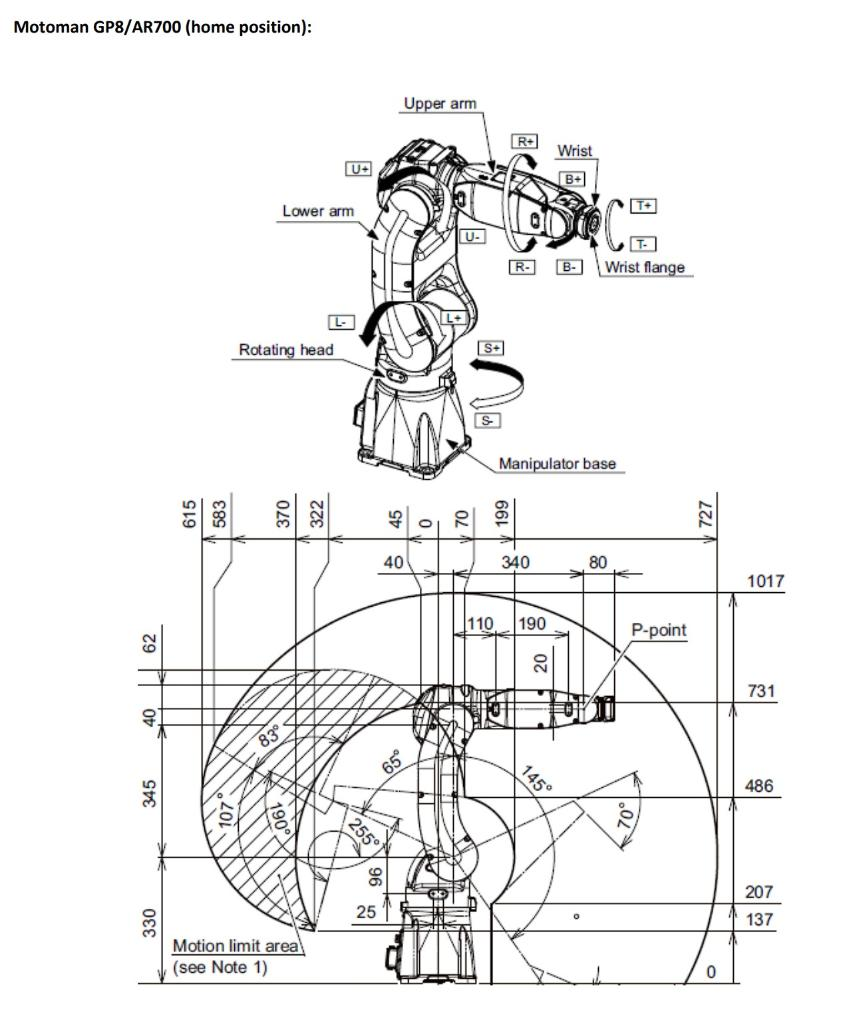
\includegraphics[scale=0.5]{robotarm.jpeg} }

\begin{table}
	\caption{Write the D-H parameters for this robot}
	\rowcolors{1}{}{gray!7}
	\begin{tabular}[t]{lccccccc}
		Link & Theta & D 	  & Radius & Alpha \\ 
		S 	 & 	     &        &        &       \\	
		L 	 & 	     &        &        &       \\	
		U 	 & 	     &        &        &       \\	
		R 	 & 	     &        &        &       \\	
		B 	 & 	     &        &        &       \\	
		T 	 & 	     &        &        &       \\	
	\end{tabular}
\end{table}
\newpage

\end{document}
